\documentclass[10pt,a4paper]{article}
\usepackage[margin=1.8cm]{geometry}
\usepackage{fontspec}
\usepackage[romanian]{babel}
\usepackage{amsmath,amssymb}
\usepackage{booktabs,graphicx}
\usepackage{tikz}
\usetikzlibrary{arrows.meta}
\usepackage[colorlinks=true,linkcolor=black,urlcolor=blue!50!black]{hyperref}
\setlength{\parskip}{3pt}
\setlength{\parindent}{0pt}

\title{\vspace{-1.2cm}Clasificatori bayesieni naivi și nenaivi:\\
ghicirea mâinii unui adversar la poker\vspace{-0.3cm}}
\author{Catalin-George Tisca}
\date{\vspace{-0.6cm}}

\begin{document}
\maketitle

\paragraph{Problema.} La poker, adversarul își ascunde cărțile. Întrebarea
noastră: \emph{doar din ce face un jucător într-o mână, putem ghici cât de bune
sunt cărțile lui?}

\textbf{Pokerul pe scurt.} Jucăm Texas Hold'em cu doi jucători. Fiecare
primește două cărți pe care doar el le vede; apoi urmează patru runde de
pariuri: \emph{preflop} (înainte de cărțile comune), \emph{flop}, \emph{turn}
și \emph{river}. La rândul lui, un jucător poate face \emph{fold} (renunță și
pierde ce a pariat), \emph{check/call} (continuă fără să mărească miza) sau
\emph{bet/raise} (mărește miza). Înainte de cărți, unul dintre jucători pune o
miză obligatorie mică, \emph{small blind}, și vorbește primul; celălalt pune
una mare, \emph{big blind}.

\textbf{Clasa} $C$ este cât de bune sunt cele două cărți: \emph{slabă},
\emph{medie} sau \emph{puternică}. O stabilim cu \emph{scorul Chen}, o formulă
simplă folosită de jucători (de exemplu A-A are 20 de puncte, iar 7-2 de culori
diferite are 1,5 puncte sub zero), cu praguri care împart toate cele 1326 de perechi posibile
de cărți aproximativ în treimi. \textbf{Caracteristicile} sunt: poziția $S$
(1 dacă e small blind, 0 dacă e big blind) și, pentru fiecare rundă $t=0,1,2,3$, ce a făcut
jucătorul, $R_t$: \emph{nimic} (nu a ajuns să acționeze), \emph{fold},
\emph{check/call} sau \emph{bet/raise} (dacă a făcut mai multe, o păstrăm pe
cea mai agresivă).

\paragraph{Date.} Folosim 40 de meciuri de câte 3000 de mâini dintre programe
de poker, din Annual Computer Poker Competition 2011 (setul public PHH, Zenodo,
DOI 10.5281/zenodo.10796885). Aceste jurnale păstrează cărțile ambilor
jucători chiar și când cineva face fold, deci știm mereu clasa corectă. Fiecare
mână dă două înregistrări, câte una pentru fiecare jucător: $240{.}000$ în
total. Concursul joacă aceleași cărți de două ori, cu locurile schimbate, așa
că împărțim datele după grupul de cărți, ca o mână și „geamăna'' ei să ajungă
mereu de aceeași parte: aproximativ 70\% pentru antrenare ($180{.}000$) și
30\% pentru test ($60{.}000$), aleși aleator cu \texttt{seed=0}.

\paragraph{Cele două modele.} Ambele învață probabilitățile prin simplă
numărare în datele de antrenare (adăugăm 1 la fiecare numărătoare, ca nicio
probabilitate să nu iasă 0) și aleg, cu regula lui Bayes, clasa cea mai
probabilă având caracteristicile observate. Diferă doar ce depinde de ce
(săgețile din figură):
\begin{center}
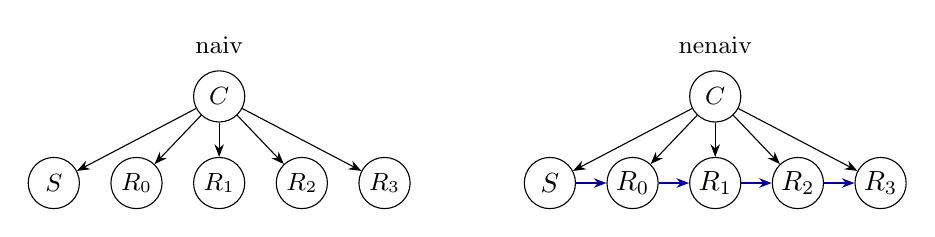
\begin{tikzpicture}[>={Stealth[length=1.6mm]},n/.style={circle,draw,minimum size=6.5mm,inner sep=0pt,font=\small},x=1.05cm]
  \node at (1.5,1.15) {\small naiv};
  \node[n] (C) at (1.5,0.5) {$C$};
  \foreach \v/\x in {S/-0.5,R_0/0.5,R_1/1.5,R_2/2.5,R_3/3.5} \node[n] (\v) at (\x,-0.6) {$\v$};
  \foreach \v in {S,R_0,R_1,R_2,R_3} \draw[->] (C) -- (\v);
  \begin{scope}[xshift=6.3cm]
  \node at (1.5,1.15) {\small nenaiv};
  \node[n] (D) at (1.5,0.5) {$C$};
  \foreach \v/\x in {Q/-0.5,S_0/0.5,S_1/1.5,S_2/2.5,S_3/3.5} \node[n] (\v) at (\x,-0.6) {};
  \node at (Q) {$S$}; \node at (S_0) {$R_0$}; \node at (S_1) {$R_1$};
  \node at (S_2) {$R_2$}; \node at (S_3) {$R_3$};
  \foreach \v in {Q,S_0,S_1,S_2,S_3} \draw[->] (D) -- (\v);
  \draw[->,thick,blue!60!black] (Q) -- (S_0); \draw[->,thick,blue!60!black] (S_0) -- (S_1);
  \draw[->,thick,blue!60!black] (S_1) -- (S_2); \draw[->,thick,blue!60!black] (S_2) -- (S_3);
  \end{scope}
\end{tikzpicture}
\end{center}
\vspace{-2mm}
\begin{align*}
\text{naiv:}\quad & P(c)\,P(s\mid c)\,P(r_0\mid c)\,P(r_1\mid c)\,P(r_2\mid c)\,P(r_3\mid c),\\
\text{nenaiv:}\quad & P(c)\,P(s\mid c)\,P(r_0\mid c,s)\,P(r_1\mid c,r_0)\,P(r_2\mid c,r_1)\,P(r_3\mid c,r_2).
\end{align*}
Modelul naiv presupune că, dacă știm clasa, ce face jucătorul într-o rundă
nu are legătură cu ce a făcut în alta. Cel nenaiv lasă fiecare acțiune să
depindă și de acțiunea din runda anterioară (iar acțiunea preflop și de
poziție), exact ca $P(\text{câștig}\mid\text{spam},\text{loterie})$ în loc de
$P(\text{câștig}\mid\text{spam})$ de la laborator.

\paragraph{Rezultate pe datele de test.} Folosim patru măsuri.
\emph{Acuratețea}: cât de des clasa aleasă e cea corectă. \emph{Log-loss}:
media lui $\ln\big(1/P(\text{clasa corectă})\big)$; e mică dacă modelul a dat
probabilitate mare răspunsului corect și foarte mare dacă a fost sigur pe el și
a greșit. \emph{Brier}: eroarea pătratică dintre probabilitățile date și
răspunsul corect. Pentru ultimele două, mai mic înseamnă mai bine.
\emph{Încrederea}: în medie, ce probabilitate dă modelul clasei pe care o
alege. Ca punct de comparație, „doar a priori'' ignoră acțiunile și dă mereu
frecvențele claselor (36\%, 38\%, 25\%).

\begin{center}
\begin{minipage}{0.52\textwidth}
\centering\small
\begin{tabular}{lcccc}
\toprule
model & acuratețe & log-loss & Brier & încredere\\
\midrule
doar a priori & 0{,}382 & 1{,}084 & 0{,}657 & 0{,}384\\
naiv          & 0{,}442 & 1{,}115 & 0{,}662 & 0{,}567\\
nenaiv        & \textbf{0{,}469} & \textbf{1{,}008} & \textbf{0{,}610} & 0{,}487\\
\bottomrule
\end{tabular}\\[4pt]
\begin{tabular}{lccc}
\toprule
\multicolumn{4}{l}{înregistrări cu fold preflop (6472)}\\
\midrule
model & acuratețe & log-loss & încredere\\
\midrule
naiv   & 0{,}682 & 1{,}130 & 0{,}935\\
nenaiv & 0{,}682 & 0{,}840 & 0{,}777\\
\bottomrule
\end{tabular}
\end{minipage}\hfill
\begin{minipage}{0.44\textwidth}
\centering
\includegraphics[width=\textwidth]{figures/calibration.pdf}\\[-1mm]
{\small Calibrare: dacă un model spune 70\%, ar trebui să aibă dreptate
în 70\% din cazuri (linia punctată).}
\end{minipage}
\end{center}

\textbf{Modelul nenaiv e mai bun la toate măsurile.} Ca să verificăm că nu
e noroc, refacem comparația pe 1000 de seturi de test reeșantionate
(bootstrap): în 95\% din cazuri câștigul de acuratețe e între $+2{,}3$ și
$+3{,}3$ puncte procentuale, iar log-loss-ul scade cu o valoare între $0{,}102$ și $0{,}110$.
Surpriza: modelul naiv are log-loss \emph{mai mare} decât referința care nu se
uită deloc la acțiuni, deși ghicește clasa mai des. Motivul: e prea sigur pe
el. Când spune 93\%, are dreptate doar în 68\% din cazuri (figura).

\paragraph{De unde vin diferențele.}
\begin{enumerate}\setlength{\itemsep}{1pt}
\item \textbf{Aceeași informație numărată de mai multe ori.} Cine face fold
preflop iese din mână, deci sigur nu mai acționează pe flop, turn și river
($R_1=R_2=R_3=$\,„nimic''). Modelul naiv nu știe asta. Pentru el, „nu a acționat pe
flop'' e un indiciu nou de mână slabă (probabilitate $0{,}31$ la mâinile slabe
față de $0{,}13$ la cele puternice), la fel pe turn și pe river. Așa că
numără același fold de patru ori și ajunge la o încredere de 93\%. Modelul
nenaiv învață că după un fold „nimic'' urmează sigur, oricare ar fi cărțile
($P\approx1$ pentru toate clasele), deci rundele lipsă nu mai adaugă nimic:
aceeași acuratețe (68\%), dar o încredere de 78\%, apropiată de realitate.
\item \textbf{Acțiunile se leagă și prin stilul jucătorului, nu doar prin
cărți.} Un jucător agresiv pariază și preflop, și pe flop, oricare i-ar fi
cărțile. Pentru modelul naiv, un bet pe flop e de $2{,}1$ ori mai probabil cu o
mână puternică decât cu una slabă ($0{,}50$ față de $0{,}24$). Modelul nenaiv
știe dacă jucătorul a pariat deja preflop; în acest caz raportul e doar
$1{,}3$ ($0{,}61$ față de $0{,}46$). Deci un bet pe flop după un raise preflop
spune mult mai puțin decât crede modelul naiv, care îl adaugă peste indiciul
deja numărat.
\item \textbf{O caracteristică inutilă singură devine utilă în combinație.}
Poziția nu spune nimic despre cărți: fiecare clasă e small blind în 50\% din
cazuri. Dar un fold preflop înseamnă altceva în fiecare poziție. Cu o mână
slabă, small blind-ul face fold în 34\% din cazuri, big blind-ul doar în 9\%
(el a pus deja miza mare și adesea poate continua gratuit). Modelul naiv
folosește aceeași valoare, 22\%, pentru amândoi și pierde această diferență.
\end{enumerate}
\paragraph{Pe scurt.} Câștigul la acuratețe e modest (+2,8 puncte), pentru
că de multe ori ambele modele aleg aceeași clasă; diferența mare e în cât de
corecte sunt probabilitățile. Când caracteristicile depind unele de altele,
modelul naiv numără aceeași informație de mai multe ori și devine prea sigur;
modelul nenaiv învață aceste legături și rămâne realist. Ambele ghicesc corect
doar în jur de 47\% din cazuri: acțiunile depind mult și de cărțile comune de
pe masă, pe care niciun model nu le vede. Clasele nu sunt perfect egale (36\%,
38\%, 25\%), pentru că scorul Chen ia puține valori.

\paragraph{Cum se rulează.} \texttt{python3 bayes\_poker.py} (necesită
Python 3.9+, numpy și matplotlib). Scriptul descarcă singur datele (circa
45 MB) în \texttt{data/}, antrenează și testează ambele modele cu
\texttt{seed=0} (rezultate identice la fiecare rulare), afișează toate cifrele
din acest raport și salvează figura în \texttt{figures/calibration.pdf}.
Clasificatorii sunt scriși de la zero: aceeași clasă \texttt{BayesClassifier}
pentru ambele, care diferă doar prin lista de „părinți'' ai fiecărei
caracteristici.

\end{document}
